\documentclass[Main.tex]{TeksturSkalering}

\begin{document}

\input{txtFiles/TekstureSkalering.txt}

\lstset{numbers=left, language=[Sharp]C}
\lstinputlisting[caption = Et eksempel på en kamera klasse, label = kameraKlasse, ]{kode/Kamera.cs}


\begin{figure}[h]
\centering
\parbox{7cm}{   
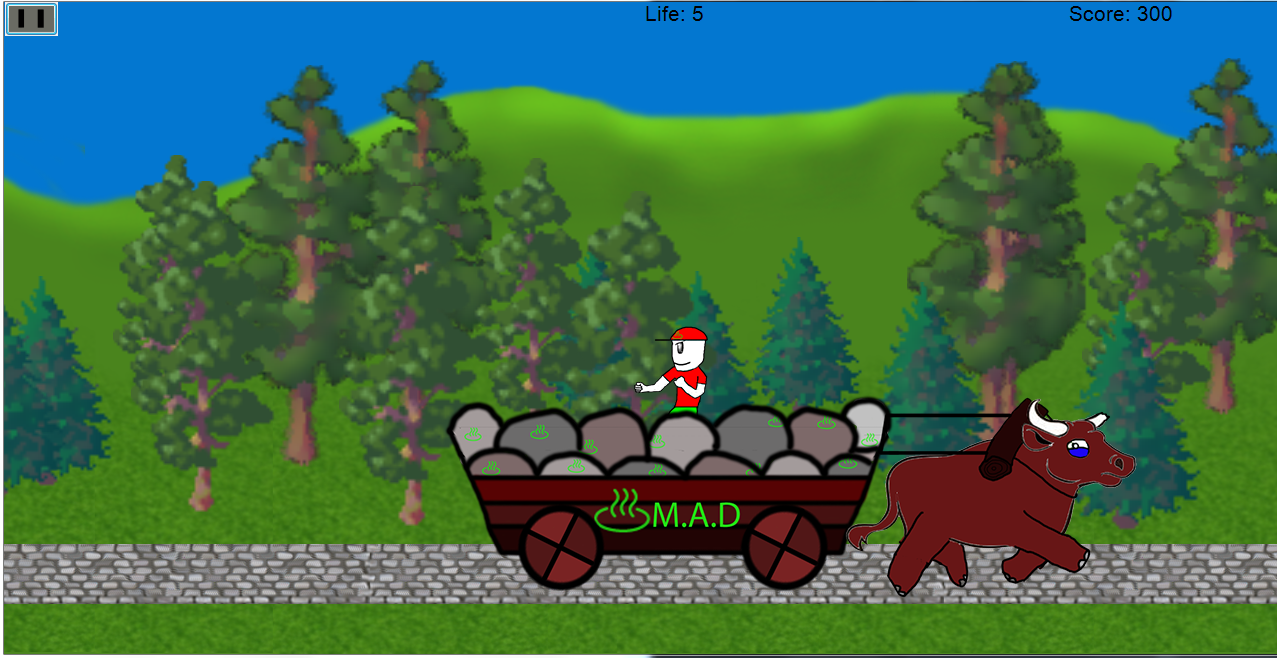
\includegraphics[width = 7cm]{billeder/MADscaling1}
\caption{MAD i produktions opløsning}    
\label{MADscaling1}}
\qquad
\begin{minipage}{7cm}
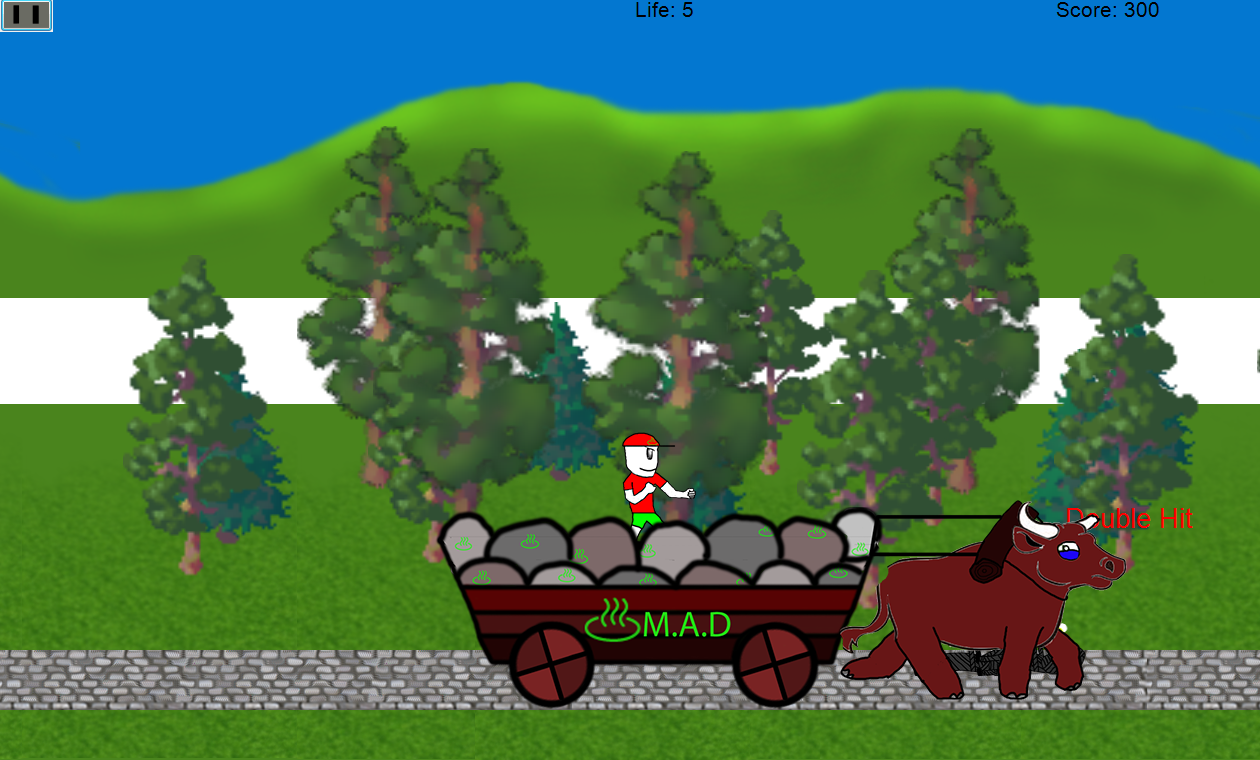
\includegraphics[width = 7cm]{billeder/MADscaling2}
\caption{MAD i 1280x800 opløsning med skærm kordinator}    
\label{MADscaling2}
\end{minipage}
\end{figure}

\begin{figure}[h]
\centering
\parbox{7cm}{   
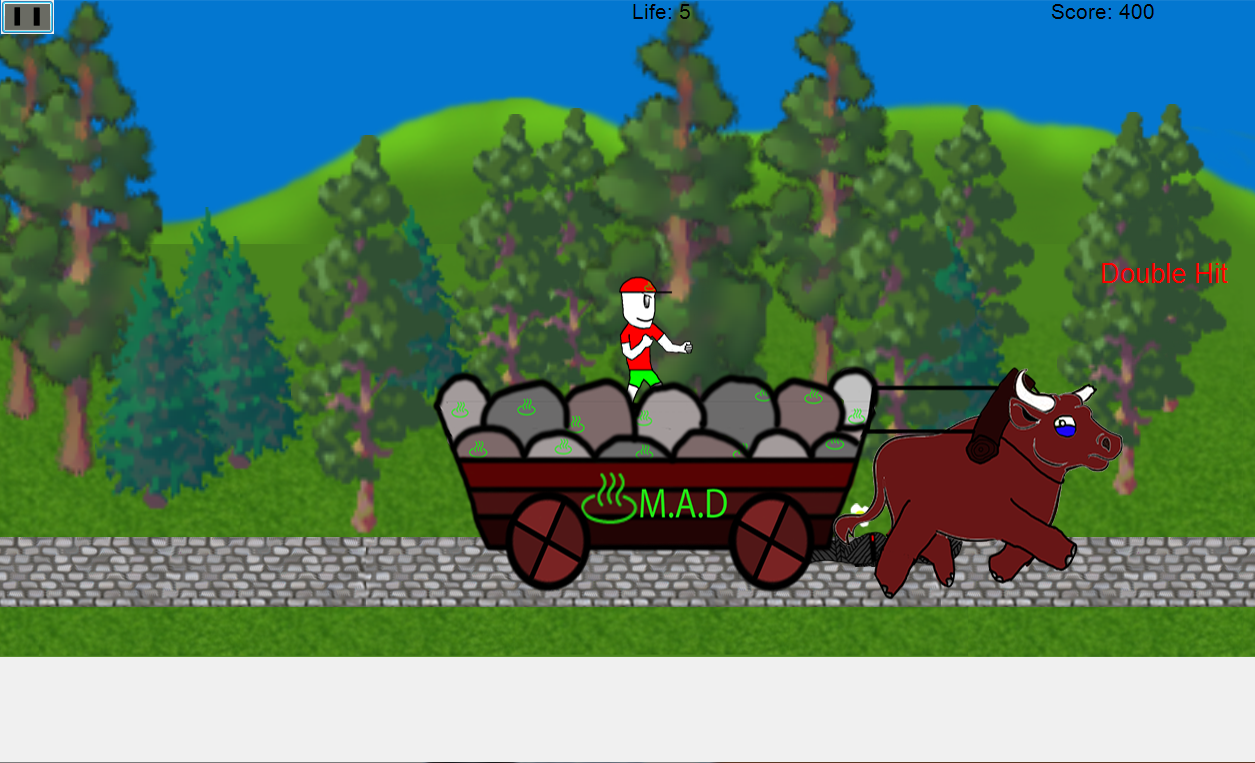
\includegraphics[width = 7cm]{billeder/MADscaling3}
\caption{MADscaling3}    
\label{MADscaling3}}
\qquad
\begin{minipage}{7cm}

\includegraphics[width = 7cm]{billeder/MADscaling4}
\caption{MADscaling4}    
\label{MADscaling4}
\end{minipage}
\end{figure}

\begin{figure}
\centering
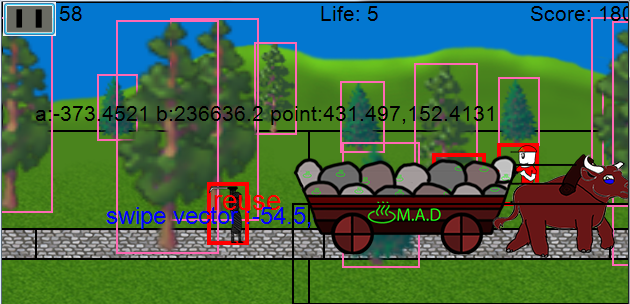
\includegraphics[width = 7 cm]{billeder/MADscaling5}
\caption{derb}
\label{MADscaling5}
\end{figure}

\begin{figure}
\centering
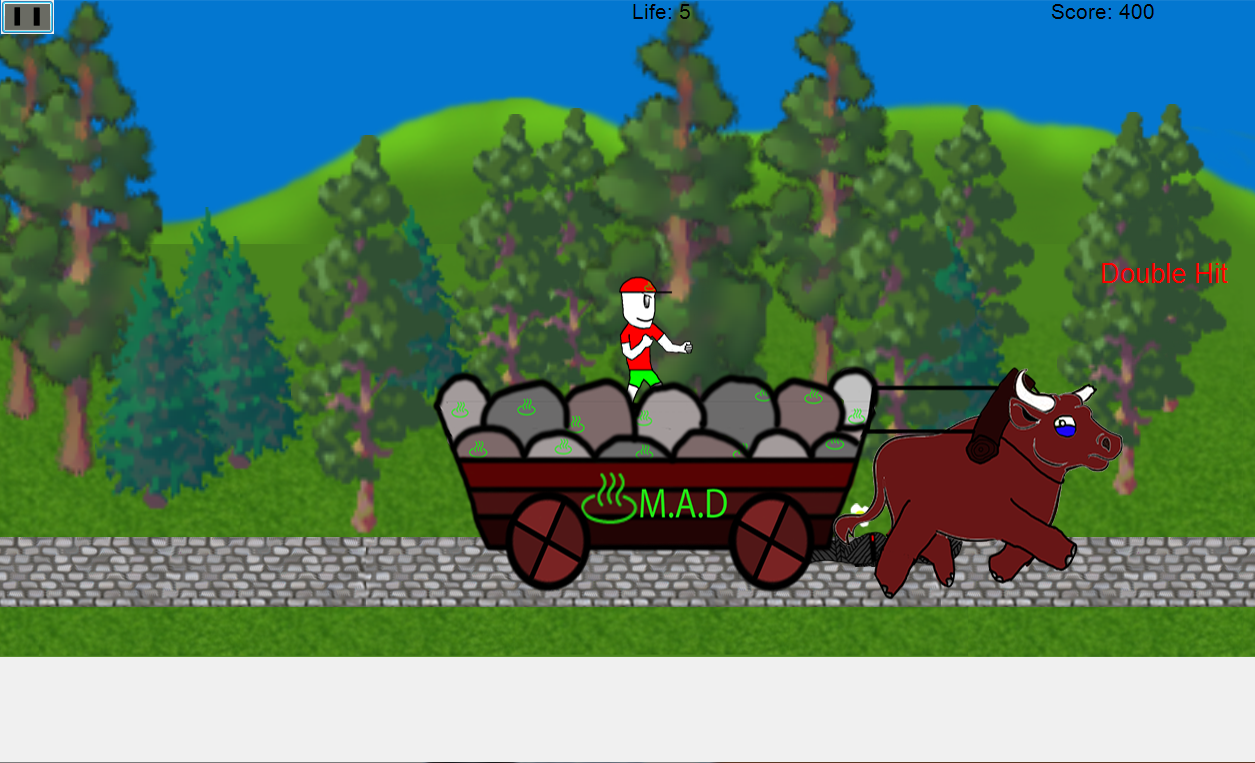
\includegraphics[width = 7 cm]{billeder/MADscaling6}
\caption{derbo}
\label{MADscaling6}
\end{figure}

\end{document}